\documentclass{ximera}
%% You can put user macros here
%% However, you cannot make new environments

\usepackage[letterpaper, total={6in, 8in}]{geometry}

\usepackage{tikz}
\usepackage{tkz-euclide}
\usetkzobj{all}

\tikzstyle geometryDiagrams=[ultra thick,color=blue!50!black]

%\usepackage{enumerate}
\usepackage{euler}

 
\usetikzlibrary{shapes,snakes}
\tikzset{
  dot hidden/.style={},
  line hidden/.style={},
  dot colour/.style={dot hidden/.append style={color=#1}},
  dot colour/.default=black,
  line colour/.style={line hidden/.append style={color=#1}},
  line colour/.default=black
}

%\begin{sagesilent}
def mydata(k):
    import numpy as np
    # Random test data
    np.random.seed(123)
    all_data = [np.random.normal(0, std, 100) for std in range(1, k)]
    return all_data

#boxplot
def seabox(my_data,mystr):
    import seaborn as sns
    sns.set_style("whitegrid")
    #tips = sns.load_dataset("tips")
    ax = sns.boxplot(x=my_data)
    ax.set(xlim=(0, None))    
    ax.get_figure().savefig(mystr,bbox_inches='tight')

#histogram
def myhist(k,b,m,M):
    from sage.plot.histogram import Histogram
    #k=data size
    # b= number of bins
    # random datA range
    a=histogram([randint(m,M) for _ in range(k)], bins=b)
    return a

#barchart & table
'''data1=[
['Zoo','giraffes', 'orangutans', 'monkeys'], ['SF Zoo', 20, 14, 23],['LA Zoo',12, 18, 29]
]'''
def mytb(data1,table_name,bar_name):
    import plotly.plotly as py
    import plotly.graph_objs as go
    from plotly.tools import FigureFactory as FF 
    from IPython.display import Image

    table1=FF.create_table(data1)
    py.iplot(table1,filename=table_name[:-4])
    py.image.save_as(table1, filename=table_name)
    Image(table_name)
    width=len(data1[0])
    height=len(data1)
    show(width)
    trace=[]
    d0=data1[0][1:width]
    show(d0)
    for i in range(height-1):
        show(i)
        d1=data1[i+1][1:width]
        show(d1)
        trace.append(
            go.Bar(
            x=d0,
            y=d1,
            name=data1[i+1][0]
                   )
                     )
    data = trace
    layout = go.Layout(
        barmode='group'
    )

    fig = go.Figure(data=data, layout=layout)
    py.iplot(fig, filename=bar_name[:-4])
    py.image.save_as(fig, filename=bar_name)
    Image(bar_name)
#piechart :
def mypie(labels,values,pie_name):
    import plotly.plotly as py
    import plotly.graph_objs as go
    from IPython.display import Image
    trace=go.Pie(labels=labels,values=values)
    py.iplot([trace], filename=data_name[:-4])
    py.image.save_as([trace],filename=pie_name)
    Image(pie_name)
    
\end{sagesilent}



\title{Statistics Visuals HW}
\author{Oguz Kurt}
\begin{document}
\begin{abstract}
\empty
\end{abstract}
\maketitle
\begin{sagesilent}
def mydata(k):
    import numpy as np
    # Random test data
    np.random.seed(123)
    all_data = [np.random.normal(0, std, 100) for std in range(1, k)]
    return all_data

#boxplot
def seabox(my_data,mystr):
    import seaborn as sns
    sns.set_style("whitegrid")
    #tips = sns.load_dataset("tips")
    ax = sns.boxplot(x=my_data)
    ax.set(xlim=(0, None))    
    ax.get_figure().savefig(mystr,bbox_inches='tight')

#histogram
def myhist(k,b,m,M):
    from sage.plot.histogram import Histogram
    #k=data size
    # b= number of bins
    # random datA range
    a=histogram([randint(m,M) for _ in range(k)], bins=b)
    return a

#barchart & table
'''data1=[
['Zoo','giraffes', 'orangutans', 'monkeys'], ['SF Zoo', 20, 14, 23],['LA Zoo',12, 18, 29]
]'''
def mytb(data1,table_name,bar_name):
    import plotly.plotly as py
    import plotly.graph_objs as go
    from plotly.tools import FigureFactory as FF 
    from IPython.display import Image

    table1=FF.create_table(data1)
    py.iplot(table1,filename=table_name[:-4])
    py.image.save_as(table1, filename=table_name)
    Image(table_name)
    width=len(data1[0])
    height=len(data1)
    show(width)
    trace=[]
    d0=data1[0][1:width]
    show(d0)
    for i in range(height-1):
        show(i)
        d1=data1[i+1][1:width]
        show(d1)
        trace.append(
            go.Bar(
            x=d0,
            y=d1,
            name=data1[i+1][0]
                   )
                     )
    data = trace
    layout = go.Layout(
        barmode='group'
    )

    fig = go.Figure(data=data, layout=layout)
    py.iplot(fig, filename=bar_name[:-4])
    py.image.save_as(fig, filename=bar_name)
    Image(bar_name)
#piechart :
def mypie(labels,values,pie_name):
    import plotly.plotly as py
    import plotly.graph_objs as go
    from IPython.display import Image
    trace=go.Pie(labels=labels,values=values)
    py.iplot([trace], filename=data_name[:-4])
    py.image.save_as([trace],filename=pie_name)
    Image(pie_name)
    
\end{sagesilent}




\begin{problem} Below, you will find the box plot of the total bill of customers dining in the restaurant ``Yeah Me Too!'' throughout a single week. Please, answer the following questions.

\begin{image}
    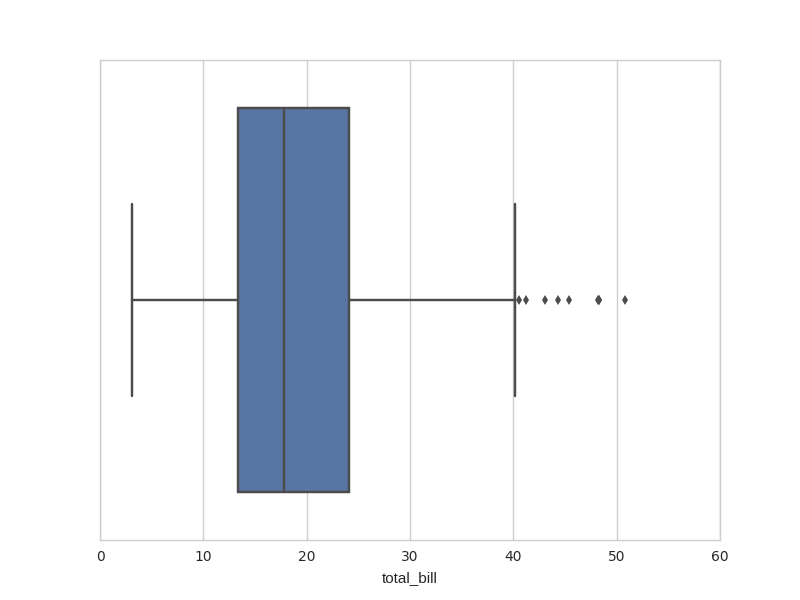
\includegraphics[width=15cm]{../img/hbplot.png}
\end{image}

\begin{enumerate}
    \item What is the median?
 \begin{multipleChoice}
    \choice{6}
    \choice{14}
    \choice[correct]{18}
    \choice{24}
    \choice{55}
\end{multipleChoice}
    \item What is the 1st Quartile?
 \begin{multipleChoice}
    \choice{6}
    \choice[correct]{14}
    \choice{18}
    \choice{24}
\end{multipleChoice}
    \item What is the 3rd Quartile?
 \begin{multipleChoice}
    \choice{14}
    \choice{18}
    \choice[correct]{24}
    \choice{30}
    \choice{40}
\end{multipleChoice}
    \item What is the IQR?
 \begin{multipleChoice}
    \choice{3}
    \choice[correct]{10}
    \choice{14}
    \choice{15}
\end{multipleChoice}
    \item What is the minimum?
 \begin{multipleChoice}
    \choice{0}
    \choice[correct]{3}
    \choice{6}
    \choice{14}
\end{multipleChoice}
    \item What is the maximum?
 \begin{multipleChoice}
    \choice{40}
    \choice{50}
    \choice[correct]{52}
    \choice{55}
\end{multipleChoice}
    \item Is the left end of the whisker minimum or (1st Quartile)-1.5*(IQR)?
    \begin{hint}
        Whiskers are the thin lines that end at a hash mark on both ends of the box. Outliers are the small dots outside them.
    \end{hint}
 \begin{multipleChoice}
    \choice[correct]{Minimum}
    \choice{(1st Quartile)-1.5*(IQR)}
\end{multipleChoice}
    \item Is the right end of the whisker maximum or (3rd Quartile)+1.5*(IQR)?
    \begin{hint}
        Whiskers are the thin lines that end at a hash mark on both ends of the box. Outliers are the small dots outside them.
    \end{hint}
 \begin{multipleChoice}
    \choice{Maximum}
    \choice[correct]{(3rd Quartile)+1.5*(IQR)}
\end{multipleChoice}

\end{enumerate}
\end{problem}

\begin{problem}
\begin{sagesilent}
import numpy as np
data=[1,24,25,30,31,35,45, 50, 50, 50 , 52, 52, 65, 65, 76, 77, 78, 78, 78, 78, 80, 83, 85, 86, 89, 90, 90, 90, 99,100]

def myperc(data,p):
    n=len(data)
    if 0<=p and p<=100:
        l=p*(n+1)/100
        f=l.floor()
        r=l-f
        if f<n:
            new=data[f-1]+r*(data[f]-data[f-1])
            show(new)
            return new
        else:
            return data[n-1]
    else:
        return "percent must be between 0 and 100."
\end{sagesilent}
Please, draw the box plot representing the following sample data consisting of 30 exam scores in a class of 100 students and \textbf{submit it in class on Monday}. Moreover, answer the following problems.

$$\sage{data}$$

\begin{enumerate}
    \item Minimum is $\answer{\sage{min(data)}}$.
    \item Maximum is $\answer{\sage{max(data)}}$.
    \item Mode is $\answer{\sage{mode(data)[0]}}$.
    \item Median is $\answer{\sage{myperc(data,50)}}$.
    \item 1st Quartile is $\answer{\sage{myperc(data,25)}}$.
    \item 3rd Quartile is $\answer{\sage{myperc(data,75)}}$.
    \item 71th--percentile is $\answer{\sage{myperc(data,71)}}$.
    \item Sample Mean is $\answer[tolerance=0.01]{\sage{mean(data)}}$.
    \item Sample Variance is $\answer[tolerance=0.01]{\sage{variance(data)}}$.
    \item Sample Standard Deviation is $\answer[tolerance=0.01]{\sage{std(data)}}$.
\end{enumerate}
\end{problem}


\begin{problem}
\begin{sagesilent}
import scipy.stats
data=[6,24,25,30,31,35,45]
\end{sagesilent}
Please, draw the box plot representing the following sample data consisting of 30 exam scores in a class of 100 students and \textbf{submit it in class on Monday}. Moreover, answer the following problems.

$$\sage{data}$$

\begin{enumerate}
    \item Minimum is $\answer{\sage{min(data)}}$.
    \item Maximum is $\answer{\sage{max(data)}}$.
    \item Mode is $\answer{\sage{mode(data)[0]}}$.
    \item Median is $\answer{\sage{myperc(data,50)}}$.
    \item 1st Quartile is $\answer{\sage{myperc(data,25)}}$.
    \item 3rd Quartile is $\answer{\sage{myperc(data,75)}}$.
    \item 71th--percentile is $\answer{\sage{myperc(data,71)}}$.
    \item Sample Mean is $\answer[tolerance=0.01]{\sage{mean(data)}}$.
    \item Sample Variance is $\answer[tolerance=0.01]{\sage{variance(data)}}$.
    \item Sample Standard Deviation is $\answer[tolerance=0.01]{\sage{std(data)}}$.
\end{enumerate}
\end{problem}


\begin{problem}
\begin{sagesilent}
import scipy.stats
data=[9,10,16,16,32,32,48,50]
\end{sagesilent}
Please, draw the box plot representing the following sample data consisting of 30 exam scores in a class of 100 students and \textbf{submit it in class on Monday}. Moreover, answer the following problems.

$$\sage{data}$$

\begin{enumerate}
    \item Minimum is $\answer{\sage{min(data)}}$.
    \item Maximum is $\answer{\sage{max(data)}}$.
    \item Mode is $\answer{\sage{mode(data)[0]}}$.
    \item Median is $\answer{\sage{myperc(data,50)}}$.
    \item 1st Quartile is $\answer{\sage{myperc(data,25)}}$.
    \item 3rd Quartile is $\answer{\sage{myperc(data,75)}}$.
    \item 71th--percentile is $\answer{\sage{myperc(data,71)}}$.
    \item Sample Mean is $\answer[tolerance=0.01]{\sage{mean(data)}}$.
    \item Sample Variance is $\answer[tolerance=0.01]{\sage{variance(data)}}$.
    \item Sample Standard Deviation is $\answer[tolerance=0.01]{\sage{std(data)}}$.
\end{enumerate}
\end{problem}

\begin{problem}
\begin{sagesilent}
size=50
bin=7
min=10
max=50
data_list=[17, 42, 41, 28, 37, 23, 50, 43, 48, 44, 48, 14, 37, 27, 21, 14, 41, 11, 39, 22, 37, 44, 40, 23, 43, 49, 31, 18, 10, 34, 22, 50, 14, 40, 10, 33, 24, 26, 12, 40, 21, 37, 20, 13, 35, 42, 10, 19, 16, 40]
data_list.sort()
myxmin=data_list[0]
myxmax=data_list[size-1]


seahist(data_list,bin,"hist1.png")

\end{sagesilent}

The following is the histogram of exam scores of a sample of $\sage{size}$ students. Please, answer the questions.


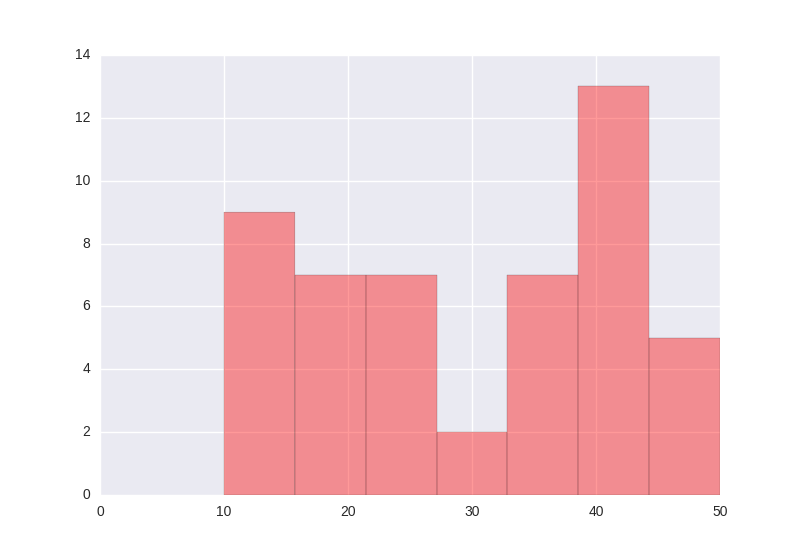
\includegraphics[width=12cm]{hist1.png}

\begin{enumerate}
    \item Minimum exam score is $\answer[tolerance=2]{\sage{myxmin}}$
    \item Maximum exam score is $\answer[tolerance=2]{\sage{myxmax}}$
    \item Number of bins is $\answer{\sage{bin}}$.
    \item Length of each subinterval is $\answer[tolerance=0.5]{\sage{myxmax/bin-myxmin/bin}}$
%    \item Size of data is $\answer[tolerance=4]{\sage{size}}$
\end{enumerate}
\end{problem}


\begin{problem}
\begin{sagesilent}
size=100
bin=6
min=25
max=100
data_list1=[95, 97, 43, 68, 77, 93, 81, 89, 87, 80, 81, 96, 68, 34, 31, 79, 45, 91, 97, 92, 37, 35, 33, 44, 61, 96, 99, 81, 71, 80, 41, 66, 39, 74, 52, 30, 44, 67, 60, 97, 70, 66, 29, 27, 46, 83, 93, 42, 66, 51, 42, 99, 57, 99, 27, 60, 51, 55, 71, 75, 26, 43, 32, 59, 41, 92, 76, 34, 49, 62, 40, 88, 57, 83, 88, 52, 33, 40, 87, 69, 88, 83, 91, 67, 41, 52, 51, 27, 69, 40, 92, 98, 93, 95, 92, 94, 73, 77, 80, 76]
data_list1.sort()    
seahist(data_list1,bin,"hist2.png")
myxmin=data_list1[0]
myxmax=data_list1[size-1]
\end{sagesilent}

The following is the histogram of exam scores of a sample of $\sage{size}$ students. Please, answer the questions.

%\sageplot[width=12cm][png]{myhis}

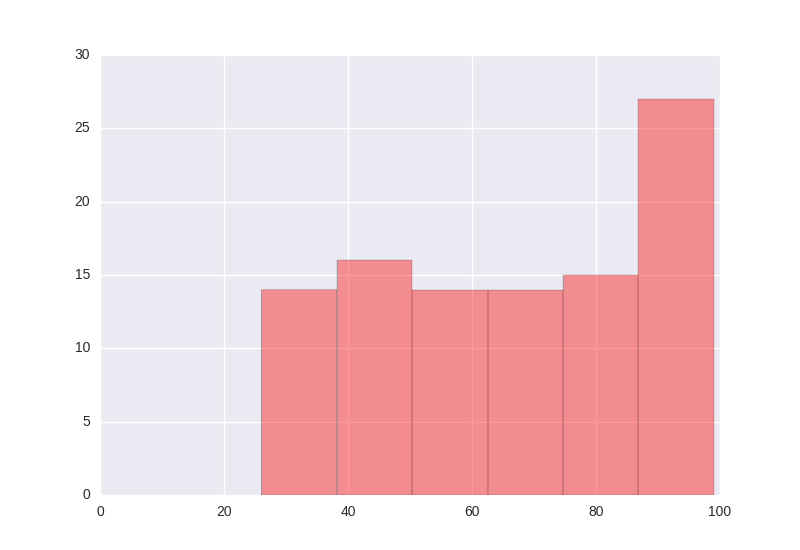
\includegraphics[width=12cm]{hist2.png}

\begin{enumerate}
    \item Minimum exam score is $\answer[tolerance=2]{\sage{myxmin}}$
    \item Maximum exam score is $\answer[tolerance=2]{\sage{myxmax}}$
    \item Number of bins is $\answer{\sage{bin}}$.
    \item Length of each subinterval is $\answer[tolerance=0.5]{\sage{myxmax/bin-myxmin/bin}}$
%    \item Size of data is $\answer[tolerance=4]{\sage{size}}$
\end{enumerate}
\end{problem}


\begin{problem}
The following is the histogram of exam scores of a sample of 70 students. Please, answer the questions.

\begin{sagesilent}
size=50
bin=6
mydata=[30, 36, 28, 28, 27, 29, 22, 29, 40, 23, 30, 35, 24, 33, 33, 27, 32,
       28, 22, 32, 33, 34, 36, 32, 29, 31, 27, 29, 38, 25, 31, 32, 22, 31,
       29, 36, 26, 29, 32, 29, 23, 28, 29, 33, 32, 29, 31, 36, 26, 27]
mydata.sort()    
seahist(mydata,bin,"hist3.png")
myxmin=mydata[0]
myxmax=mydata[size-1]
\end{sagesilent}

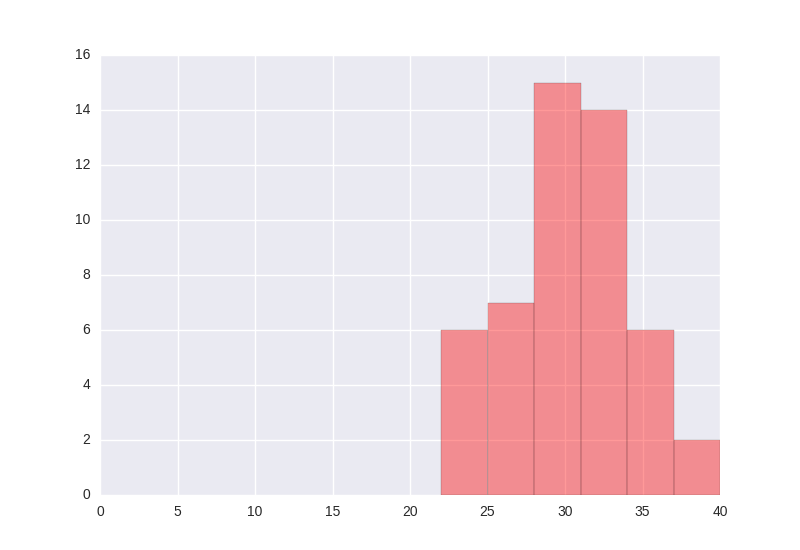
\includegraphics[width=12cm]{hist3.png}

\begin{enumerate}
    \item Minimum exam score is $\answer[tolerance=2]{\sage{myxmin}}$
    \item Maximum exam score is $\answer[tolerance=2]{\sage{myxmax}}$
    \item Number of bins is $\answer{\sage{bin}}$.
    \item Length of each subinterval is $\answer[tolerance=0.5]{\sage{myxmax/7-myxmin/7}}$
%    \item Size of data is $\answer[tolerance=4]{\sage{size}}$
\end{enumerate}
\end{problem}


\begin{problem}
\begin{sagesilent}
mydata=[10,14,15,16,16,18,21,24,24,25,26,28,28,29,29,30,30,32,32,32,36,37,40,40,42,42,43,44,49,50]
mydata.sort()
bin=5
min=mydata[0]
max=mydata[len(mydata)-1]
bin=5
binsize=(max-min)/bin
ind=[min+i*binsize for i in range(bin+1)]
subd=[[x for x in mydata if (x<ind[i+1] and x>= ind[i]) or (i==bin-1 and x==max)] for i in range(bin)]
\end{sagesilent}

Draw the histogram of the following data set using $\sage{bin}$ bins. Submit your work in class on Monday!

$$\sage{mydata}$$

\begin{enumerate}
    \item Minimum is $\answer{\sage{min}}$.
    \item Maximum is $\answer{\sage{max}}$.
    \item The width of each bin is $\answer[tolerance=0.01]{\sage{binsize}}$.
    \item Bin 1 corresponds to data whose values are in the interval 
    $[\answer{\sage{ind[0]}}, \answer[tolerance=0.01]{\sage{ind[1]}})$
    \item The number of data in bin 1 is $\answer[tolerance=0.01]{\sage{len(subd[0])}}$.
    \item Bin 2 corresponds to data whose values are in the interval 
    $[\answer[tolerance=0.01]{\sage{ind[1]}}, \answer[tolerance=0.01]{\sage{ind[2]}})$
    \item The number of data in bin 2 is $\answer[tolerance=0.01]{\sage{len(subd[1])}}$
    \item Bin 3 corresponds to data whose values are in the interval 
    $[\answer[tolerance=0.01]{\sage{ind[2]}}, \answer[tolerance=0.01]{\sage{ind[3]}})$
    \item The number of data in bin 3 is $\answer[tolerance=0.01]{\sage{len(subd[2])}}$
    \item Bin 4 corresponds to data whose values are in the interval 
    $[\answer[tolerance=0.01]{\sage{ind[3]}}, \answer[tolerance=0.01]{\sage{ind[4]}})$
    \item The number of data in bin 4 is $\answer[tolerance=0.01]{\sage{len(subd[3])}}$
    \item Bin 5 corresponds to data whose values are in the interval 
    $[\answer[tolerance=0.01]{\sage{ind[4]}}, \answer[tolerance=0.01]{\sage{ind[5]}}]$
    \item The number of data in bin 5 is $\answer{\sage{len(subd[4])}}$
    \item Now that you answered, almost all relevant questions, please submit the sketch of the histogram in class.
\end{enumerate}
\end{problem}


\begin{problem}
\begin{sagesilent}
mydata=[5,8,8,8,8,12,15,18,18,19,19,22,23,25,25,25,27,31,31,32,32,32,32,33,35,39,40,49,50,51,52,52,53,53,54]
mydata.sort()
min=mydata[0]
max=mydata[len(mydata)-1]
bin=6
binsize=(max-min)/bin
ind=[min+i*binsize for i in range(bin+1)]
subd=[[x for x in mydata if (x<ind[i+1] and x>= ind[i]) or (i==bin-1 and x==max)] for i in range(bin)]
\end{sagesilent}

Draw the histogram of the following data set using $\sage{bin}$ bins. Submit your work in class on Monday!

$$\sage{mydata}$$

\begin{enumerate}
    \item Minimum is $\answer{\sage{min}}$.
    \item Maximum is $\answer{\sage{max}}$.
    \item The width of each bin is $\answer[tolerance=0.01]{\sage{binsize}}$.
    \item Bin 1 corresponds to data whose values are in the interval 
    $[\answer[tolerance=0.01]{\sage{ind[0]}}, \answer[tolerance=0.01]{\sage{ind[1]}})$
    \item The number of data in bin 1 is $\answer{\sage{len(subd[0])}}$.
    \item Bin 2 corresponds to data whose values are in the interval 
    $[\answer[tolerance=0.01]{\sage{ind[1]}}, \answer[tolerance=0.01]{\sage{ind[2]}})$
    \item The number of data in bin 2 is $\answer{\sage{len(subd[1])}}$
    \item Bin 3 corresponds to data whose values are in the interval 
    $[\answer[tolerance=0.01]{\sage{ind[2]}}, \answer[tolerance=0.01]{\sage{ind[3]}})$
    \item The number of data in bin 3 is $\answer{\sage{len(subd[2])}}$
    \item Bin 4 corresponds to data whose values are in the interval 
    $[\answer[tolerance=0.01]{\sage{ind[3]}}, \answer[tolerance=0.01]{\sage{ind[4]}})$
    \item The number of data in bin 4 is $\answer{\sage{len(subd[3])}}$
    \item Bin 5 corresponds to data whose values are in the interval 
    $[\answer[tolerance=0.01]{\sage{ind[4]}}, \answer[tolerance=0.01]{\sage{ind[5]}})$
    \item The number of data in bin 5 is $\answer{\sage{len(subd[4])}}$
    \item Bin 6 corresponds to data whose values are in the interval 
    $[\answer[tolerance=0.01]{\sage{ind[5]}}, \answer[tolerance=0.01]{\sage{ind[6]}}]$
    \item The number of data in bin 5 is $\answer{\sage{len(subd[4])}}$
    \item Now that you answered, almost all relevant questions, please submit the sketch of the histogram in class.
\end{enumerate}
\end{problem}



\end{document}
